% EnergyPilot: documents A and B (CSE 406, Phase 2 Term Project)
% Build: pdflatex main.tex (run twice). Also works on Overleaf (IEEEtran is built in).
\documentclass[conference,a4paper]{IEEEtran}
\IEEEoverridecommandlockouts

\usepackage[T1]{fontenc}
\usepackage[utf8]{inputenc}
\usepackage{textcomp}
\usepackage{cite}
\usepackage{amsmath,amssymb}
\usepackage{booktabs}
\usepackage{array}
\usepackage{tikz}
\usetikzlibrary{arrows.meta,positioning,fit,backgrounds}
\usepackage{algorithmicx}
\usepackage{algpseudocode}
\usepackage[hyphens]{url}
\urlstyle{same}
\def\BibTeX{{\rm B\kern-.05em{\sc i\kern-.025em b}\kern-.08em
    T\kern-.1667em\lower.7ex\hbox{E}\kern-.125emX}}

% ---- project info (change here) ----
\newcommand{\groupname}{Group EnergyPilot}

% ---- compact pseudocode blocks ----
\algrenewcommand\algorithmicindent{0.9em}
\algrenewcommand\alglinenumber[1]{\scriptsize #1:}
\newenvironment{pseudo}
  {\par\vspace{2pt}\noindent\begin{minipage}{\columnwidth}\hrule\vspace{2pt}\footnotesize\begin{algorithmic}[1]}
  {\end{algorithmic}\vspace{1pt}\hrule\end{minipage}\par\vspace{5pt}}

\begin{document}
\pagestyle{plain}

\title{EnergyPilot: A Proactive Agentic Home Energy Optimizer}

\author{
\IEEEauthorblockN{Emil Ljungdell}
\IEEEauthorblockA{\textit{\groupname}\\Hanyang University}
\and
\IEEEauthorblockN{Philip Dahlensj\"o}
\IEEEauthorblockA{\textit{\groupname}\\Hanyang University}
\and
\IEEEauthorblockN{Filip Kadmark}
\IEEEauthorblockA{\textit{\groupname}\\Hanyang University}
\and
\IEEEauthorblockN{Jasmin Hansson}
\IEEEauthorblockA{\textit{\groupname}\\Hanyang University}
}

\maketitle

\begin{abstract}
EnergyPilot is a proposal for a software agent that runs household appliances at the cheapest suitable time, without the resident having to program anything. The resident states an intent, for example ``the laundry should be done by 07:00, and keep the cost low'', and the agent turns it into a schedule based on forecast electricity prices and household usage. It acts on its own or asks for approval, explains every decision, and plans again when prices or devices change. This document extends our requirement document with the specification phase. It lists eleven requirements in one list, describes the development environment (a Python and TypeScript web application in Linux containers, with an estimated cost of at most 44 USD), reviews the software and algorithms we build on, and specifies at pseudocode level how each requirement will be implemented. The first version uses simulated appliances and synthetic or public data behind a device interface that can later be replaced by real devices.
\end{abstract}

\begin{IEEEkeywords}
smart home, agentic AI, energy optimization, requirements, specification, scheduling
\end{IEEEkeywords}

\begin{table}[t]
\caption{Role assignments (till the middle of the term)}
\label{tab:roles}
\centering
\footnotesize
\setlength{\tabcolsep}{3pt}
\begin{tabular}{@{}p{0.2\columnwidth}p{0.2\columnwidth}p{0.5\columnwidth}@{}}
\toprule
\textbf{Roles} & \textbf{Name} & \textbf{Task description}\\
\midrule
User & Philip Dahlensj\"o & Sets intents and preferences, tries the prototype and reports usability problems.\\
Customer & Emil Ljungdell & Represents the household that pays the bill. Prioritizes the requirements and accepts the result.\\
Software developer & Jasmin Hansson & Designs and implements the agent, the scheduler, the backend and the user interface.\\
Development manager & Filip Kadmark & Tracks deadlines, leads group meetings, follows up tasks and makes sure each deliverable is submitted.\\
\bottomrule
\end{tabular}
\end{table}

\section{Introduction}

\subsection{Motivation}
Electricity prices change during the day, but most households run their appliances when it suits them, which is often when power is expensive. Moving flexible loads such as laundry and dishwashing to cheaper hours lowers the bill and can also ease the peak load on the grid. Doing this by hand takes effort: you need to know the prices, remember to start the machine and be at home when it is time. We think an agent can do this for the resident. It also matches this year's course topic, a proactive agentic home that predicts, decides and acts before a problem occurs.

\subsection{Problem Statement and Client Needs}
The client is a household that pays the electricity bill and owns several connected appliances. Its needs are:
\begin{itemize}
\item lower electricity cost without losing convenience (the laundry must still be done when the resident needs it),
\item no manual programming of schedules or rules,
\item full control, so the resident can always override the agent,
\item understandable decisions, so the resident can see why the agent did something, and
\item careful handling of usage data, since it shows when people are home.
\end{itemize}

\subsection{Related Software}
\textbf{LG ThinQ} lets users control LG appliances remotely, build smart routines and monitor energy use, including a comparison with neighbors and savings goals with notifications \cite{lgthinq}. The routines are built by the user, and the energy features mainly report what has already happened.

\textbf{Samsung SmartThings Energy} has an AI Energy Mode that adjusts supported Samsung appliances and TVs to use less energy on selected cycles, and an Away mode for turning devices off when nobody is home \cite{stnews,stsupport}. The optimization mostly happens inside each device.

\textbf{Google Home} shows energy history and an energy dashboard for Nest thermostats, with separate heating and cooling totals, and the Nest Learning Thermostat builds a schedule from the household's routine \cite{nest,nestnews}. The energy functions we found are centered on the thermostat.

\textbf{Matter} is a connectivity standard that lets devices from different brands work together \cite{matter}. It is relevant if EnergyPilot is later connected to real devices.

In the material we found, none of these products lets the user state an intent (a deadline and a cost preference) that an agent turns into a schedule across several appliances based on electricity prices. We will verify this in the apps before the final report.

\subsection{Scope}
The first version covers scheduling of flexible appliances (washing machine, dryer, dishwasher and one climate device), price and usage forecasting, a user interface for intents and overrides, and a savings report. Real hardware, billing integration and solar production are out of scope for now.

\section{Requirements}
The requirements are given in one list. Each is prioritized as Must or Should and can change during the project. Section~\ref{sec:spec} specifies how each requirement is achieved, in the same order.

\subsection{R1: Appliance registration and device interface (Must)}
The user registers an appliance with its type, power in watts, typical cycle length and earliest start. All appliances are accessed through one device interface, so simulated appliances can later be replaced by real ones without changing the rest of the system.

\subsection{R2: Intent input (Must)}
The user states a goal as free text, such as ``done by 07:00'' or ``cheapest possible today'', or with a simple form. The system shows how it understood the goal and asks for confirmation. A new user can register an appliance and set an intent in under five minutes.

\subsection{R3: Electricity prices (Must)}
The system gets hourly prices for the next 24 to 48 hours from a price source behind one interface. The first source is a synthetic time-of-use tariff, and public price data can be added through the same interface.

\subsection{R4: Price and usage forecasting (Should)}
The system predicts hourly prices and household consumption for the coming day. It compares several forecasting methods on past data and uses the one with the lowest error.

\subsection{R5: Schedule generation (Must)}
For each intent the agent chooses the start time with the lowest cost that respects the deadline, the quiet hours and the maximum household load. A schedule for the next 24 hours is ready in under 10 seconds, and a plan that breaks a hard constraint is never executed.

\subsection{R6: Act or ask (Should)}
The user chooses, per appliance, whether the agent starts it automatically or asks for approval first.

\subsection{R7: Decision log and explanations (Must)}
Every decision is saved with a short explanation in plain language, for example ``Started the washer at 02:00, 38\,\% cheaper than 18:00''. The numbers in an explanation always come from the scheduler.

\subsection{R8: Savings dashboard (Should)}
A dashboard shows consumption, cost and estimated savings compared with a baseline without the agent.

\subsection{R9: Manual override (Must)}
The user can change, cancel or start a planned run at any time. Manual control always wins over the agent.

\subsection{R10: Replanning (Should)}
If prices change or an appliance goes offline, the agent makes a new plan for the runs that have not started and tells the user.

\subsection{R11: Security and privacy (Must)}
Login is required, communication is encrypted, and only the data needed for scheduling is stored. The user can delete all of their own data.

\section{Development Environment}

\subsection{Choice of Software Development Platform}
\textbf{Platform.} EnergyPilot is a web application. The backend runs in Linux containers (Docker), and the user interface runs in any modern browser on a phone or a computer. We chose the web because the user installs nothing, the same build works on every operating system, and a demo only needs a browser. We rejected a native mobile app, because builds and test devices would take time that we need for the agent itself.

\textbf{Programming languages.} The backend, the forecasting and the scheduler are written in Python 3.12. We need its data libraries (pandas, NumPy, scikit-learn), which we also use in the AI course, and FastAPI gives us a typed REST API that generates its own documentation. The frontend uses TypeScript with React, because type checking catches mistakes in the data we get from the API.

\textbf{Version control and documents.} The code and this document are in a public GitHub repository, \url{https://github.com/PhilipDahlensjo/SE-AI_project}. The documents are LaTeX files in the repository (IEEEtran, also usable in Overleaf). We track work with issues and pull requests, and each issue names the requirement it implements.

\textbf{Development environment.} Table~\ref{tab:env} lists what we use. Exact library versions are fixed in the lock files in the repository.

\begin{table}[t]
\caption{Development environment}
\label{tab:env}
\centering
\footnotesize
\setlength{\tabcolsep}{3pt}
\begin{tabular}{@{}p{0.27\columnwidth}p{0.67\columnwidth}@{}}
\toprule
\textbf{Item} & \textbf{Choice}\\
\midrule
Developer machines & \textbf{[TODO: each member adds OS version, CPU and RAM]}\\
Server OS & Ubuntu Linux LTS in Docker containers\\
Backend & Python 3.12, FastAPI, Pydantic v2\\
Database & PostgreSQL 16 (SQLite in unit tests), SQLAlchemy 2\\
Data and ML & pandas, NumPy, scikit-learn\\
Frontend & TypeScript 5, React, Vite\\
Containers & Docker and Docker Compose\\
Tests and CI & pytest, GitHub Actions\\
LLM & LLM API with tool calling, used only to read the intent and to word explanations\\
Documents & LaTeX (IEEEtran), Overleaf\\
\bottomrule
\end{tabular}
\end{table}

\textbf{Cloud (bonus).} We plan to deploy on AWS Lightsail with the Small-2GB Linux plan (2 vCPU, 2~GB RAM, 60~GB storage, 12 USD per month), running the backend, the database and the frontend with Docker Compose \cite{lightsail}. Developers also run the same Compose file locally.

\textbf{Cost estimation.} Table~\ref{tab:cost} shows the estimate. All software is free or open source, and we need no new hardware. The LLM cost is a limit, not a price: we set a spending limit of 20 USD in the provider's console, and the usage (a few hundred short requests per week) should stay far below it.

\begin{table}[t]
\caption{Cost estimation}
\label{tab:cost}
\centering
\footnotesize
\begin{tabular}{@{}lr@{}}
\toprule
\textbf{Item} & \textbf{USD}\\
\midrule
Open-source software, GitHub, Overleaf (free plans) & 0\\
Developer computers (already owned) & 0\\
AWS Lightsail Small-2GB, about 2 months & 24\\
LLM API usage (spending limit) & $\le$ 20\\
\midrule
\textbf{Total} & $\le$ \textbf{44}\\
\bottomrule
\end{tabular}
\end{table}

\subsection{Software in Use}
Products that do a similar task are described in Section~I-C. None of them schedules several appliances from a stated intent. We build on the following existing software and algorithms:
\begin{itemize}
\item \emph{Seasonal naive forecast}, which predicts the value from 24 hours earlier \cite{hyndman}, as the baseline forecaster.
\item \emph{Ridge regression} and \emph{gradient boosting} \cite{friedman} from scikit-learn \cite{sklearn} for price and consumption forecasts.
\item \emph{Exhaustive search} over start slots in the scheduler. If a household load limit makes several appliances depend on each other, the CP-SAT solver in OR-Tools \cite{ortools} is the next step.
\item \emph{FastAPI} \cite{fastapi} for the REST API.
\item \emph{LLM tool calling} \cite{claudedocs} to turn the resident's text into structured data.
\item Later, optionally, the \emph{LG ThinQ Connect API} \cite{thinqconnect} and \emph{Matter} \cite{matter} for real appliances.
\end{itemize}

\subsection{Task Distribution}
As the assignment allows, the task distribution will be given in the design document (C). The roles until then are in Table~\ref{tab:roles}.

\section{Specifications}\label{sec:spec}
Fig.~\ref{fig:overview} shows how the parts fit together, and Table~\ref{tab:data} lists the main data. Time is divided into 15-minute slots ($\Delta t = 0.25$ h), so 48 hours are 192 slots. Each subsection below belongs to the requirement with the same number in Section~II.

\begin{figure}[t]
\centering
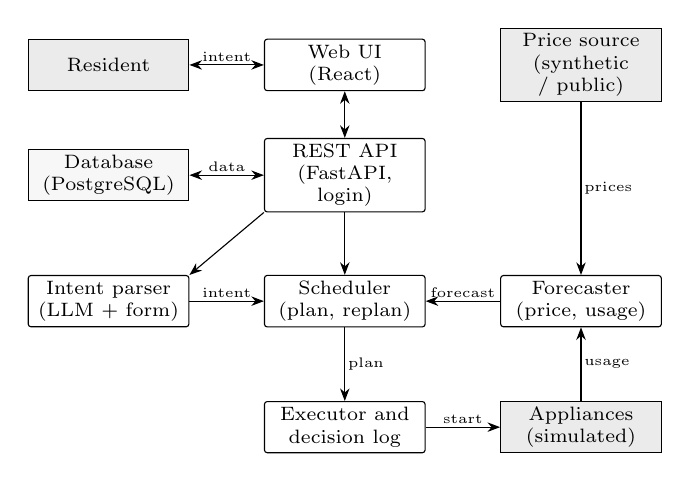
\begin{tikzpicture}[font=\scriptsize, >={Stealth[length=1.6mm]},
  lab/.style={font=\tiny, inner sep=1pt},
  box/.style={draw, rounded corners=1pt, align=center, minimum height=6.5mm, inner sep=2pt, text width=1.9cm},
  ext/.style={draw, align=center, minimum height=6.5mm, inner sep=2pt, fill=black!8, text width=1.9cm},
  db/.style={draw, align=center, minimum height=6.5mm, inner sep=2pt, text width=1.9cm, fill=black!3}]
\node[ext] (res) at (0,4.6) {Resident};
\node[box] (ui)  at (3.0,4.6) {Web UI\\(React)};
\node[ext] (src) at (6.0,4.6) {Price source\\(synthetic / public)};
\node[box] (api) at (3.0,3.2) {REST API\\(FastAPI, login)};
\node[db]  (dbs) at (0,3.2) {Database\\(PostgreSQL)};
\node[box] (intent) at (0,1.6) {Intent parser\\(LLM + form)};
\node[box] (sched) at (3.0,1.6) {Scheduler\\(plan, replan)};
\node[box] (fore) at (6.0,1.6) {Forecaster\\(price, usage)};
\node[box] (exec) at (3.0,0) {Executor and\\decision log};
\node[ext] (dev) at (6.0,0) {Appliances\\(simulated)};
\draw[<->] (res) -- node[above,lab]{intent} (ui);
\draw[<->] (ui) -- (api);
\draw[<->] (api) -- node[above,lab]{data} (dbs);
\draw[->] (src) -- node[right,lab]{prices} (fore);
\draw[->] (api.south west) -- (intent.north east);
\draw[->] (api) -- (sched);
\draw[->] (intent) -- node[above,lab]{intent} (sched);
\draw[->] (fore) -- node[above,lab]{forecast} (sched);
\draw[->] (sched) -- node[right,lab]{plan} (exec);
\draw[->] (exec) -- node[above,lab]{start} (dev);
\draw[->] (dev) -- node[right,lab]{usage} (fore);
\end{tikzpicture}
\caption{System overview: main parts and data flows.}
\label{fig:overview}
\end{figure}

\begin{table}[t]
\caption{Main data}
\label{tab:data}
\centering
\footnotesize
\setlength{\tabcolsep}{3pt}
\begin{tabular}{@{}p{0.2\columnwidth}p{0.74\columnwidth}@{}}
\toprule
\textbf{Entity} & \textbf{Main fields}\\
\midrule
User & id, e-mail, password hash\\
Device & id, user, type, power (W), cycle (min), mode (auto/ask), adapter\\
Intent & id, device, earliest start, deadline, goal (cheapest/fastest), status\\
Price & slot start, price per kWh (relative unit in synthetic data)\\
Consumption & slot start, kWh, source\\
Run & id, device, intent, start, cost, baseline cost, status, manual flag\\
DecisionLog & time, run, action, explanation text\\
\bottomrule
\end{tabular}
\end{table}

\subsection{R1: Appliance registration and device interface}
A device is stored with its data, and every action goes through an adapter that has the same three operations for simulated and real appliances. The simulated adapter runs a cycle on the simulator clock.
\begin{pseudo}
\Procedure{RegisterDevice}{$u, spec$}
\State check $spec.power > 0$ and $spec.cycle \ge 15$ min
\State $d \gets$ \Call{Save}{Device($u$, $spec$)}
\State $d.adapter \gets$ \Call{AdapterFor}{$spec.adapter$} \Comment{simulated by default}
\State \Return $d$
\EndProcedure
\Statex
\State \textbf{interface} DeviceAdapter: \textsc{state}(), \textsc{start}(), \textsc{stop}()
\end{pseudo}

\subsection{R2: Intent input}
The LLM only converts text to a fixed JSON format (device, deadline, goal). The result is checked against a schema, and a plain form is the fallback, so the demo also works without the LLM.
\begin{pseudo}
\Procedure{SetIntent}{$u, text$}
\State $j \gets$ \Call{LLMParse}{$text$} \Comment{JSON: device, deadline, goal}
\If{LLM unavailable \textbf{or} $j$ does not match schema}
  \State $j \gets$ \Call{AskForm}{$u$} \Comment{fallback}
\EndIf
\State show $j$ in plain words
\If{user does not confirm}
  \State \Return
\EndIf
\State $i \gets$ \Call{Save}{Intent($u, j$, pending)}
\State \Call{Plan}{$i$}
\EndProcedure
\end{pseudo}

\subsection{R3: Electricity prices}
Prices are read from the database first and fetched from the price source only if slots are missing. The synthetic tariff has three price levels over the day plus noise.
\begin{pseudo}
\Procedure{GetPrices}{$t_0, H$} \Comment{$H$ = 48 h}
\State $p \gets$ \Call{Load}{prices in $[t_0, t_0+H)$}
\If{$p$ is complete}
  \State \Return $p$
\EndIf
\State $p \gets source.$\Call{Fetch}{$t_0, H$}
\For{each slot $t$ with $p_t$ missing or $p_t < 0$}
  \State $p_t \gets p_{t-1}$ \Comment{last known value}
\EndFor
\State \Call{Save}{$p$}; \Return $p$
\EndProcedure
\Statex
\Procedure{SyntheticTariff}{$t$}
\State $k \gets$ level of hour($t$) in \{off-peak, mid, peak\}
\State \Return $base[k] \cdot (1+\varepsilon)$, $\varepsilon \sim \mathcal{N}(0,\sigma^2)$
\EndProcedure
\end{pseudo}

\subsection{R4: Price and usage forecasting}
We compare three methods with the last seven days as validation data and use the one with the lowest mean absolute error. This component is shared with our project in the AI course, which uses public price and consumption data (see the repository).
\begin{pseudo}
\Procedure{Forecast}{$hist$} \Comment{next 24 h}
\State train $\gets hist$ without last 7 days; val $\gets$ last 7 days
\For{$m \in \{$SeasonalNaive, Ridge, GradientBoosting$\}$}
  \State fit $m$ on train; features: hour, weekday, $y_{t-24}$, $y_{t-168}$
  \State $err[m] \gets$ MAE($m$.predict(val), val)
\EndFor
\State $m^* \gets \arg\min_m err[m]$; refit $m^*$ on all of $hist$
\State \Return $m^*$.predict(next 24 h), $err$
\EndProcedure
\end{pseudo}

\subsection{R5: Schedule generation}
For one appliance the agent tries every allowed start slot and keeps the cheapest. The cost of a start slot $s$ for an appliance with power $P$ and a cycle of $L$ slots, using price $c_t$, is
\begin{equation}
C(s) = \sum_{t=s}^{s+L-1} c_t \, P \, \Delta t .
\end{equation}
With 192 slots the search is far below 10 seconds. With several intents, the one with the least slack ($deadline - earliest - L$) is planned first, and each result is added to the load $l_t$.
\begin{pseudo}
\Procedure{Plan}{$i$}
\State $d \gets i.device$; $L \gets \lceil d.cycle/15 \rceil$; $P \gets d.power$
\State $c \gets$ \Call{GetPrices}{now, 48 h}; $l \gets$ load of other planned runs
\State $best \gets \bot$; $bestCost \gets \infty$
\For{$s \gets i.earliest$ \textbf{to} $i.deadline - L$}
  \If{slots $s..s+L-1$ touch quiet hours}
    \State \textbf{continue}
  \EndIf
  \If{$\exists t:\ l_t + P > L_{max}$}
    \State \textbf{continue}
  \EndIf
  \State $C \gets \sum_{t=s}^{s+L-1} c_t P \Delta t$
  \If{$C < bestCost$}
    \State $best \gets s$; $bestCost \gets C$
  \EndIf
\EndFor
\If{$best = \bot$}
  \State mark $i$ infeasible; tell the user; \Return
\EndIf
\State \textbf{assert} \Call{HardRulesOK}{$best$}
\State \Return \Call{Save}{Run($d$, $best$, $bestCost$)}
\EndProcedure
\end{pseudo}

\subsection{R6: Act or ask}
A dispatcher runs every minute. A run is only executed after the hard rules are checked again, because prices or the state of the appliance may have changed.
\begin{pseudo}
\Procedure{Dispatch}{} \Comment{every minute}
\For{each planned run $r$ with $r.start - now \le \delta$}
  \If{$r.device.mode = $ auto}
    \State \Call{Execute}{$r$}
  \Else
    \State \Call{AskUser}{$r$} \Comment{once}
    \If{approved}
      \State \Call{Execute}{$r$}
    \ElsIf{declined \textbf{or} no answer at $r.start$}
      \State cancel $r$; \Call{Log}{$r$, ``not started''}
    \EndIf
  \EndIf
\EndFor
\EndProcedure
\Statex
\Procedure{Execute}{$r$}
\If{\Call{HardRulesOK}{$r$} \textbf{and} adapter.state $=$ idle}
  \State adapter.start(); $r.status \gets$ running; \Call{Log}{$r$}
\Else
  \State \Call{Replan}{$r$}
\EndIf
\EndProcedure
\end{pseudo}

\subsection{R7: Decision log and explanations}
The explanation is first made from a template with numbers from the scheduler. The LLM may reword it, but the new text is only used if it contains no number that is missing in the original.
\begin{pseudo}
\Procedure{Explain}{$r$}
\State $base \gets$ cost if started at the earliest allowed time
\State $pct \gets 100\,(base - r.cost)/base$
\State $text \gets$ \Call{Template}{$r.device$, $r.start$, $pct$}
\If{LLM available}
  \State $t' \gets$ \Call{LLMReword}{$text$}
  \If{every number in $t'$ is in $text$}
    \State $text \gets t'$
  \EndIf
\EndIf
\State \Call{Save}{DecisionLog(now, $r$, $text$)}
\EndProcedure
\end{pseudo}

\subsection{R8: Savings dashboard}
The baseline is a resident without the agent, who starts each run at the earliest time the intent allows. The saving is
\begin{equation}
S = 100\,\frac{C_{base} - C_{agent}}{C_{base}}\ \%.
\end{equation}
\begin{pseudo}
\Procedure{Report}{$u, from, to$}
\State $R \gets$ finished runs of $u$ in $[from, to]$
\State $C_{agent} \gets \sum_{r \in R} r.cost$; $C_{base} \gets \sum_{r \in R} r.baseCost$
\State $S \gets 100\,(C_{base} - C_{agent}) / C_{base}$
\State \Return daily series (cost, baseline, kWh) and $S$
\EndProcedure
\end{pseudo}

\subsection{R9: Manual override}
A run that is already going can only be stopped, because a washing cycle cannot be moved. After any change the agent plans the other runs again, since the load has changed.
\begin{pseudo}
\Procedure{Override}{$r, action$} \Comment{cancel, move($t$), start now}
\If{$r$ is running \textbf{and} $action \ne$ cancel}
  \State \Return error
\EndIf
\State apply $action$ through the adapter; $r.manual \gets$ true
\State \Call{Log}{$r$, ``changed by user''}
\State \Call{Replan}{other planned runs}
\EndProcedure
\end{pseudo}

\subsection{R10: Replanning}
Planning is triggered by events. Runs that are manual or already running are never touched.
\begin{pseudo}
\Procedure{OnEvent}{$e$} \Comment{price update, device offline, deadline change}
\State $A \gets$ planned runs affected by $e$, sorted by slack
\For{$r \in A$ \textbf{with not} $r.manual$}
  \State $r' \gets$ \Call{Plan}{$r.intent$} \Comment{current prices}
  \If{no plan found}
    \State mark $r$ infeasible; notify the user
  \ElsIf{$r'.start \ne r.start$}
    \State update $r$; notify the user; \Call{Log}{$r$, $e$}
  \EndIf
\EndFor
\EndProcedure
\end{pseudo}

\subsection{R11: Security and privacy}
Passwords are stored as Argon2id hashes, requests carry a short-lived token, and TLS is terminated at a reverse proxy with a free certificate. Only 15-minute consumption values are kept.
\begin{pseudo}
\Procedure{Login}{$email, pw$}
\If{Argon2id.verify($user.hash$, $pw$)}
  \State \Return token($user$, expires in 1 h)
\EndIf
\State \Return error
\EndProcedure
\Statex
\Procedure{Handle}{$request$}
\State verify token
\If{$resource.owner \ne token.user$}
  \State \Return 403
\EndIf
\EndProcedure
\Statex
\Procedure{DeleteMyData}{$u$}
\State delete devices, intents, runs, consumption and log of $u$
\EndProcedure
\end{pseudo}

\begin{thebibliography}{00}
\bibitem{lgthinq} LG Electronics, ``LG ThinQ'' (app description). Accessed: Nov. 5, 2026. [Online]. Available: \url{https://www.apkmirror.com/apk/lgelectronics/lg-smartthinq}
\bibitem{stnews} SmartThings, ``New SmartThings Energy features take home energy management to next level,'' Samsung Newsroom, Jun. 27, 2023. Accessed: Nov. 5, 2026. [Online]. Available: \url{https://news.samsung.com/us/samsung-new-smartthings-energy-features-take-home-energy-management-next-level}
\bibitem{stsupport} Samsung, ``How to use SmartThings AI energy saving features.'' Accessed: Nov. 5, 2026. [Online]. Available: \url{https://www.samsung.com/ie/support/apps-services/how-to-use-smartthings-ai-energy-saving-controls/}
\bibitem{nest} Google, ``Nest Thermostat,'' Google Store. Accessed: Nov. 5, 2026. [Online]. Available: \url{https://store.google.com/product/nest_thermostat?hl=en-us}
\bibitem{nestnews} ``Google Home app update brings new features for smart thermostats,'' Notebookcheck. Accessed: Nov. 5, 2026. [Online]. Available: \url{https://www.notebookcheck.net/Google-Home-App-update-brings-new-features-for-smart-thermostats.1098863.0.html}
\bibitem{matter} Connectivity Standards Alliance, ``Matter.'' Accessed: Nov. 5, 2026. [Online]. Available: \url{https://csa-iot.org/all-solutions/matter/}
\bibitem{thinqconnect} LG Electronics, ``ThinQ Connect: Personal Access Token (PAT).'' Accessed: Nov. 5, 2026. [Online]. Available: \url{https://thinq.developer.lge.com/en/cloud/docs/thinq-connect/PAT-en}
\bibitem{hyndman} R. J. Hyndman and G. Athanasopoulos, \emph{Forecasting: Principles and Practice}, 3rd ed. Melbourne, Australia: OTexts, 2021. [Online]. Available: \url{https://otexts.com/fpp3/}
\bibitem{friedman} J. H. Friedman, ``Greedy function approximation: A gradient boosting machine,'' \emph{Ann. Statist.}, vol. 29, no. 5, pp. 1189--1232, 2001.
\bibitem{sklearn} F. Pedregosa \emph{et al.}, ``Scikit-learn: Machine learning in Python,'' \emph{J. Mach. Learn. Res.}, vol. 12, pp. 2825--2830, 2011.
\bibitem{ortools} L. Perron and V. Furnon, ``OR-Tools,'' Google. Accessed: Nov. 5, 2026. [Online]. Available: \url{https://developers.google.com/optimization/}
\bibitem{fastapi} S. Ram\'irez, ``FastAPI.'' Accessed: Nov. 5, 2026. [Online]. Available: \url{https://fastapi.tiangolo.com/}
\bibitem{claudedocs} Anthropic, ``Claude API documentation.'' Accessed: Nov. 5, 2026. [Online]. Available: \url{https://docs.claude.com}
\bibitem{lightsail} Amazon Web Services, ``Lightsail instance bundles.'' Accessed: Nov. 5, 2026. [Online]. Available: \url{https://docs.aws.amazon.com/lightsail/latest/userguide/amazon-lightsail-bundles.html}
\end{thebibliography}

\end{document}
